\documentclass[journal]{IEEEtran}

% correct bad hyphenation here
\hyphenation{op-tical net-works semi-conduc-tor}

\begin{document}

\title{Resolution-Complete Multi-agent Motion Planning with Arbitrarily-Shaped Obstacles}

\author{Biao Jia, Liang He, Dinesh Manocha}% <-this % stops a space


% The paper headers
\markboth{Final Project of comp782 motion planning}%
{Shell \MakeLowercase{\textit{et al.}}: Bare Demo of IEEEtran.cls for IEEE Journals}


% make the title area
\maketitle

% As a general rule, do not put math, special symbols or citations
% in the abstract or keywords.
\begin{abstract}
We present a novel algorithm for homogeneous multi-agent motion planning in a continuous workspace with arbitrarily-shaped obstacles. Our approach  extracts the medial-axis of the workspace and takes advantage of its geometric characteristics to spatially divide the agents into multiple clusters. For each cluster, we arrange the  agents into a circular pattern and compute their movements using a combination of inter-loop and intra-loop movements. In practice, we approximate the medial-axis and using a finite number of boundary samples to show that our planning algorithm is resolution-complete. We highlight its performance on challenging 2D benchmarks and highlight the benefits over prior methods.
\end{abstract}

% Note that keywords are not normally used for peerreview papers.
\begin{IEEEkeywords}
Multi-agent, resolution-complete, Arbirarily-Shaped, Medial-Axis.
\end{IEEEkeywords}

\IEEEpeerreviewmaketitle

\section{Introduction}
\IEEEPARstart{M}{ulti-agent} motion planning has been studied extensively in artificial intelligence, robotics and computer games.
The objective is to navigate multiple agents from a set of start positions to corresponding goal positions while avoiding inter-agent collisions as well as collisions with obstacles.
At a broad level, prior approaches can be classified into two categories: decentralized and centralized methods. 
For decentralized algorithms, the planner computes the trajectory for each agent separately for a short time horizon and uses some sort of coordination to avoid intersection between these local trajectories. On the other hand, the centralized methods combine the configuration degrees of each agent into one large high DOF (degree-of-freedom) system, which computes their paths together. Such centralized methods can provide completeness, including resolution-completeness or probabilistic-completeness guarantees. However, they are practical for scenarios with only a few low DOF agents.



%\begin{figure}[!t]
%\centering
%\includegraphics[width=2.5in]{myfigure}
% where an .eps filename suffix will be assumed under latex, 
% and a .pdf suffix will be assumed for pdflatex; or what has been declared
% via \DeclareGraphicsExtensions.
%\caption{Simulation results for the network.}
%\label{fig_sim}
%\end{figure}

\section{Prior Work}

The multi-agent path planning problem has been extensively studied in different areas. We give a brief overview of prior work in this area. 

\subsection{Decentralized Methods}
In this approach, each agent moves independently and the method computes a collision-free trajectory for a short time horizon. These techniques are commonly used in games, crowd simulation, and robotics. Some of the widely used methods are based on social forces~\cite{helbing1995social}, rule-based methods ~\cite{pelechano2007controlling}, or geometric optimization ~\cite{yeh2008composite,van2011reciprocal}, etc. However, there are no guarantees that these methods can find a collision-free solution, if one exists. Moreover, the agents can get stuck in deadlocks, though many techniques have been proposed to overcome these problems ~\cite{he2013meso,kimmel2012maintaining}. 

Another class of methods is based on decoupled algorithms. These techniques first calculate the agents' trajectories without considering each other as obstacles and then schedule their trajectories such that the agents avoid each other~\cite{cui2012pareto,sanchez2002using,peng2005coordinating,velagapudi2010decentralized}. These algorithms can handle a continuous workspace, but cannot provide completeness guarantees.  
Other decoupled algorithms ~\cite{luna2011push,de2013push,sajid2012multi} use different kind of movements when agents get close to each other. These are mostly limited to discrete workspaces.

\subsection{Centralized Methods}
These methods theoretically treat all of the agents' configurations as one unified high-DOF system and compute the collision-free paths for them. Different methods to compute the paths have been proposed. These include traditional searching ~\cite{katsev2013efficient,hart1968formal,korf1985depth,felner2012partial} and  probabilistic path planning ~\cite{carpin2002parallel,ferguson2006replanning,ferner2013odrm}. In practice, since these methods compute the paths for all agents at once, so they are limited to a few agents.
%The problem is the complexity of computation is exponentially increased with the number of agents and they usually only can handle few agents in once.

Another category of centralized methods is based on geometric decomposition techniques. ~\cite{dresner2008multiagent,calinescu2008reconfigurations,vsvestka1998coordinated} divide the workspace into several sub-areas, and agents move from one to another until they reach their goals. These algorithms control the agents' movements so that they avoid each other when they are in close proximity. While these algorithms work in a continuous workspace, the boundaries of this workspace are limited to polygonal shapes and the  complexity of the algorithms increases as a function of the number of  obstacle edges. 
%In the running stage, the computational complexity of their methods is bounded by the number of agents as well as the number of obstacles' edges. 
\cite{DBLP:journals/corr/SoloveyYZH15} present  an optimal algorithm, but the complexity is $O(n^2m^2)$, where $n$ and $m$ are the number of agents and the number of obstacles' edges, respectively. In their benchmarks, the algorithm~\cite{DBLP:journals/corr/SoloveyYZH15} takes hundreds or thousands of seconds to calculate a solution. Our approach is also a geometric decomposition method. We can handle arbitrarily-shaped obstacles and exhibit up to $100$X speedup over~\cite{DBLP:journals/corr/SoloveyYZH15}.
%In our case, the complexity in terms  number of agents and the complexity of obstacles' edges is separated. This keeps the overhead around $O(n^2)$, which means we only need to spend few seconds to simulate their benchmarks.
 


 
%\section{Background and Notation}

In this section, we introduce the notation used in the rest of the paper. We define a 2-D workspace $\mathcal{W}$, and a set of obstacles $\mathcal{O} \subseteq \mathcal{W}$. Every element in $\mathcal{O}$ can have any arbitrary shape. We assume that there are $n$ homogeneous disc-like agents, $\{\mathbf{a_{i}}, i \in [1,...n]\}$, with radius $r$ in the workspace. We use $\mathbf{p_{a_i}}$ to represent their positions. %, particularly, we use $\mathbf{p^s_a}$ to represent their start positions and $\mathbf{p^g_a}$ to represent their goal positions.
The objective of multi-agent motion planning is to find paths for all agents to goal positions from start positions while avoiding collision with each other as well as the obstacles. If there is a solution, the complete algorithms should be able to compute it.

We also define $\mathcal G$ as the extracted Blum medial-axis ~\cite{blum1978shape} from a 2-D workspace. For any point in $\mathcal G$, there are more than one closest point on the obstacles' boundaries.
According to this definition, for each point $\mathbf v \in \mathcal G$, there is a corresponding circle $A(\mathbf v,ran)$, where $\mathbf v$ is the center and $ran$ represents the radius. A circle $A(\mathbf v,ran)$ is tangent to at least two different edges of the workspace, including boundaries of obstacles . $\mathcal P(\mathbf p, \mathbf p') \subseteq \mathcal G$ represents a path in $\mathcal G$, which includes two points $\mathbf p \in \mathcal G, \mathbf p' \in \mathcal G$ and every point in between on this path of $\mathcal G$.

In this paper, we use the symbol $\mathbf{A}$ to represent one cluster of agents. For each agent $\mathbf{a} \subseteq A(\mathbf v,ran)$, we define $\mathbf{a} \in \mathbf{A}$, which means every point on the agent is covered by the corresponding $A(\mathbf v,ran)$. We can say that, if an agent $\mathbf{a} \subseteq A(\mathbf v,ran)$ then $||\mathbf{p_a} - \mathbf v|| \leq ran - r$.


If the exact medial-axis is available, we show that our algorithm is resolution-complete. In practice, most techniques compute an approximate medial-axis by taking samples on the obstacle boundaries~\cite{giesen2012medial}. As a result, our multi-agent planner is resolution-complete, as its accuracy increases with the number of samples. 
%We call our result as resolution-completeness is because the exactly medial-axis is har to be extract. But there are a lot of efficient methods can handle this problem. One of algorithm is , which it introduces a method that with increasing the number of samples(resolution) in the boundary, the accuracy of medial-axis can be increasing too. With this assumption, we call our method is resolution-completeness. 

\section{Medial-axis and Circle Packing}

Our goal is to design an algorithm for multi-agent motion planning in continuous 2D workspaces. 
%When we consider motion planning in the continuous workspace, the agents would move in the coordinates with infinite possible positions. It is hard to prove the completeness of a algorithm when agents have countless trajectories.
In our approach, we use the medial-axis of the workspace to cluster the agents.  
%e introduce an approach making use of medial-axis to cluster agents.
Theoretically, this clustering step results in  each agent being treated as a discrete element in the continuous space and also ensures that no feasible solution would be missed, up to the resolution of the medial-axis.
%in later path computing.
Overall, our algorithm uses a combination of global and local computations to compute the path for each agent.
%We can consider this algorithm containing both global and local operations.
As part of the global computation, we make use of the property of the medial-axis to divide agents into different clusters. 
As part of localized-cluster operations, we decompose $A(\mathbf v,ran)$ into several sub-areas if a large agent-cluster is associated with that region.
%The objective is to make each cluster of are strictly divided into several discrete units but does not impact the continuous feature.
Our motion planning algorithm is based on these agent clustering and area decomposition computations. Moreover, all of the agent movements (or the resulting) can be decomposed into intra-cluster and inter-cluster movements.
First, we present some theorems and lemmas to illustrate the relationship between agent positions and the medial-axis. The details related to these theorems and the proof are given in the appendix (as part of the supplementary document).
%The details of how to check whether a area of combined circles is full or not please check the supmentary document. 

\begin{theorem}
For an agent, if it does not overlap with any obstacle, there will be at least one circle $A(\mathbf v,ran)$ that includes this agent. That is, $\forall \mathbf{a}, \mathbf{a} \cap \mathcal{O} = \varnothing, \exists{ A(\mathbf v,ran)}, \mathbf{a} \subseteq  A(\mathbf v,ran)$
\label{thm:included}
\end{theorem}

We cluster all of the agents in the following manner. First, we randomly select one of the agents $\mathbf{a}$ and also select one of the points $\mathbf{v}$ on the medial-axis, that satisfy this condition $\{\mathbf{v}\ |\ argmin (||\mathbf{v} - \mathbf{p_{a}}||), \mathbf{v} \in \mathcal G\}$. 
Next, we compute an agent $\{\mathbf{a'}\ |\ argmin (||\mathbf{p_{a'}} - \mathbf{p_{a}}||)\}$. We compute a path by moving $\mathbf{v}$ along with the $\mathcal G$ toward the $\{\mathbf{v'}\ |\ argmin (||\mathbf{v'} - \mathbf{p_{a'}}||,\mathbf{v'} \in \mathcal{G})\}$, until $A(\mathbf{v},ran)$ is tangent to $\mathbf{a'}$ and we stop moving $\mathbf{v}$. In other words, if we move $\mathbf{v}$ towards $\mathbf{p_{a'}}$, then $\mathbf{a}$ won't be covered by $A(\mathbf{v},ran)$.
We compute all the agents that $\forall \mathbf{a} \subset A(\mathbf{v},ran), \mathbf{a} \in \mathbf{A_0}$. We repeat this computation till all the  agents are part of a cluster (see Algorithm \ref{algo:clusterAgents} for details). We also show the results of  clustering in Figure. \ref{fig:overview} for a simple scenarios.

\begin{algorithm}[!th]
  \SetKwInOut{Input}{input}\SetKwInOut{Output}{output}
  \Input{ A workspace $\mathcal{W}$ with a set of agents $\mathbf{a}_0, \mathbf{a}_1, ... , \mathbf{a}_n $}
  \Output{A set of clustered agents $\mathbf{A}_0, \mathbf{A}_1, ... , \mathbf{A}_m$.}
  \BlankLine
  Build the medial-axis $\mathcal{G}$ of $\mathcal{W}$
  
  $\mathcal{A}$ = All agents.
  \tcc{repeat until all the agents are clustered}
  \While{$\mathcal{A} \neq \varnothing$ }{
    Find $\mathbf{a} \in \mathcal{A}$ 
    
    Find $\{\mathbf{v}\ |\ argmin (||\mathbf{v} - \mathbf{p_{a}}||,\mathbf{v} \in \mathcal{G})\}$
    
    Find  $\{\mathbf{a'}\ |\ argmin (||\mathbf{p_{a'}} - \mathbf{p_{a}}||)\}$
    
    Find $\{\mathbf{v'}\ |\ argmin (||\mathbf{v'} - \mathbf{p_{a_n}}||,\mathbf{v'} \in \mathcal{G})\}$
    
    \While{$A(\mathbf{v},ran)$ is not tangent with $\mathbf{a}$ }{ 
    
         Move $\mathbf{v}$ along the $\mathcal{G}$ toward $\mathbf{v'}$ 
         
         \If{$\mathbf{v}$ is overlap with $\mathbf{v'}$ }{
         
            Find $\{\mathbf{a''}\ |\ argmin (||\mathbf{p_{a''}} - \mathbf{p_{a'}}||)\}$
            
            Find $\{\mathbf{v''}\ | argmin (||\mathbf{v''} - \mathbf{p_{a'}}||,\mathbf{v''} \in \mathcal{G})\}$
            
            Replace the $\mathbf{a'}$ and $\mathbf{v'}$ with $\mathbf{a''}$ and $\mathbf{v''}$ and continue. 
        }
    }
    Remove all agents $\forall \mathbf{a} \subset A(\mathbf{v},ran)$ from $\mathcal{A}$ and put them in a new cluster $\mathbf{A}$
  }
  \caption{Clustering the agents based on medial axis. This is used in Algorithm 2, Step 2.}
  \label{algo:clusterAgents}
\end{algorithm}
Moreover, we remove all the vertices from $\mathcal G$, if the radius of the corresponding circles (based on medial axis computation) is smaller than that of the agents, since no agent can be in a collision-free configuration in such circles.
\subsection{Agents Arrangement in a Cluster}

\begin{figure}[t]
\centering
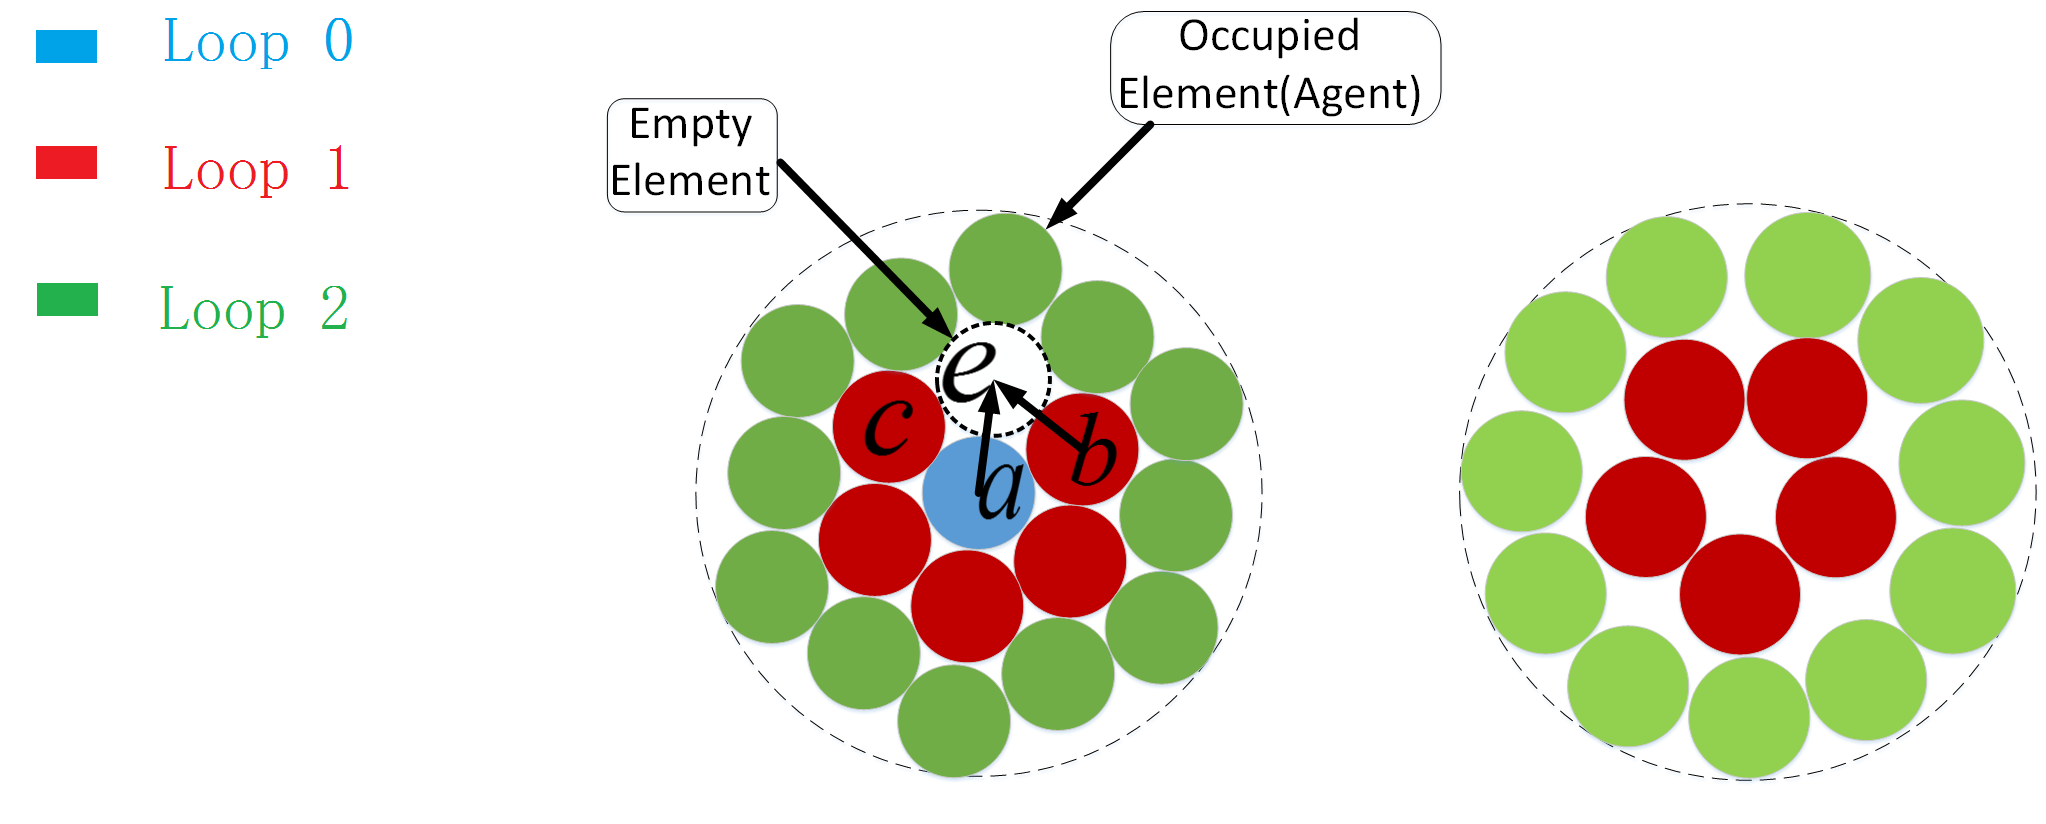
\includegraphics[width=0.7\linewidth]{figs/Fullload}
\caption{\em This figure shows a circle of the medial-axis and a set of clustered agents. The elements are arranged tightly, and we use different color to represent the elements in different loops. The dotted circle represents an empty element $\mathbf{e}$. 
%We assume two elements are connected if they can move and just touch each other. 
The two arrows, $\mathbf{a}$ to $\mathbf{e}$ and $\mathbf{b}$ to $\mathbf{e}$ show the inter-loop and intra-loop movements, respectively. The right figure shows another tight arrangement with different number of elements.}
\vspace*{-0.15in}
\label{fig:circular}
\end{figure}

In terms of efficiency, we want to use a general data structure to represent a group of clustered agents along with their incident circular area $A(\mathbf v,ran)$.
This data structure is used as a layout that arranges each agent in a certain area of the incident circle $A(\mathbf v,ran)$. In other words, any arrangement of agents in the $A(\mathbf v,ran)$ can be transitioned into this general layout. This reduces to ~\emph{circle packing}~\cite{graham1998dense} problem. It corresponds to computing how to fill a given domain with a maximum number of uniquely-sized circles.  According to ~\cite{graham1998dense} every circular area can only accommodate a certain number of agents and this number can be easily calculated. Notice that this packing arrangement for a maximum number of agents is unique, and every agent connects to at least two other agents in such an arrangement. Such an arrangement is called a \emph{tight arrangement} or a \emph{tight pattern}.
Note that when several clusters and their incident circular areas partially overlap with each other, the domain of clusters is not circle-like anymore. For example, when $ A(\mathbf v,ran) \cap A'(\mathbf v,ran) \neq \varnothing$, the shape of $ A(\mathbf v,ran) \cup A'(\mathbf v,ran)$ is not a circle.
Currently, to best of our knowledge, optimal circle packing in a domain of any shape is a difficult problem with a high complexity. ~\cite{galiev2013linear} presents an approximate method to fill the uniquely sized circles in any given domain with linear running time. In practice, their algorithm can find the approximate tight arrangement in tens of seconds. This running speed depends on the sampling resolution of the domain. We present a simplified method to compute a faster approximate solution to check if a combined circular domain is a tight arrangement in the supplemental document. In the following discussion, we first present our algorithm for a single domain.

We define two agents as connected if they can be tangent to each other along a moving path, without colliding with any other agents. We represent two such connected agents as $a \sim a'$. Assume an area with a group of disc-like agents.  
Any agent in the circle can find a path, which starts from one of it's connected agents and ends with another agent. Such a path only visits these agents once. We then call this path {\em loop} $\mathbf{T}$ . 
With these formulations, we state the following lemma. 

\vspace*{0.05in}
\begin{lemma}
Assuming an area with a group of disc-like agents, then all of the agents in the circle can find a loop. 
That is, we have: $ \forall{\mathbf{a}} \subset A(\mathbf v,ran), \exists{\mathbf{T}}, \mathbf{a} \in \mathbf{T}$
\label{lem:loop}
\end{lemma}
\vspace*{0.05in}

The proof of Lemma \ref{lem:loop} and the minimum number of connections theorems can be deducted from ~\cite{graham1998dense}.
We call the arrangement based on such a loop as the \emph{circular pattern}, which is composed of a set of \emph{elements}. This arrangement be occupied by an agent or an empty element (i.e. without an agent) in each loop.
We show two such possible layouts in Figure ~\ref{fig:circular}. 
Specifically, we label a cluster incident circle as \emph{full} if it cannot cover any new agent. 
Otherwise, it is a \emph{non-full} circle. 
Moreover, any set of clustered agents in a circle can be transited into a circular pattern by adjusting their positions if and only if the number of agents is not over the maximum capability of the area according to the analysis of ~\cite{graham1998dense}.
Based on this formulation, the overall multi-agent algorithm is given in Algorithm 2. 
Figure \ref{fig:overview} shows how to move an agent to its goal position through Algorithm \ref{algo:overview}.

\begin{algorithm}[!th]
  \SetKwInOut{Input}{input}\SetKwInOut{Output}{output}
  \Input{ A workspace $\mathcal{W}$ with a set of agents $\mathbf{a}_0, \mathbf{a}_1, ... , \mathbf{a}_n$ and their goal position 
  $\mathbf{p'}_0, \mathbf{p'}_1, ... , \mathbf{p'}_n$
  }
  \Output{Move all agents to their goal position or report no solution can be found.}
  \BlankLine
  Compute the medial-axis $\mathcal{G}$ of $\mathcal{W}$
  
  Cluster the agents according to their positions and size.
  
  \For{$\mathbf{a_i} ,i = 0, 1, 2, ... n$ }{
    Find the cluster $\mathbf{A_k}$ that $\mathbf{a_i}$ belongs to. 
    
    Find the path $\mathcal{P}$ which starts from the $\mathbf{A_k}$ and ends with $\mathbf A_{k+t}$, which includes goal position the $\mathbf{p'}_i$.
    
    \tcc{agent moves from cluster $\mathbf{A_k}$ to $\mathbf A_{k+t}$}
    
    \For{All clusters that $\mathcal{P}$ overlaps with}{
        $\mathbf{a_i}$ moves using the intra-loop and inter-loop exchange algorithm. 
    }
    \tcc{Now agent $\mathbf{a_i} \subseteq \mathbf{A}_{k+t}$ and move to its goal position }  
    
     $\mathbf{a_i}$ moves to $\mathbf{p'}_i$ using intra-loop and inter-loop exchange algorithm.
  }
 
  
  \caption{Multi-Agent Planning Overall Algorithm}
  \label{algo:overview}
\end{algorithm}

\section{Element Movements}

In this section we show how to move an element, that is performed as part of the intra-loop and inter-loop exchange algorithms (Algorithm 2, Steps 7 and 8). We first present the theorem, which illustrates the spatial relationship of two nearby elements' movements. 
\begin{theorem}
An element $\mathbf{c}$ can be moved to another nearby element$\mathbf{c'}$'s position 
if and only if both of them are connected to an empty element 
or at least one of them, $\mathbf{c}$ or $\mathbf{c'}$ is empty. 
\label{thm:min}
\end{theorem}
\begin{figure}[!ht]
\centering
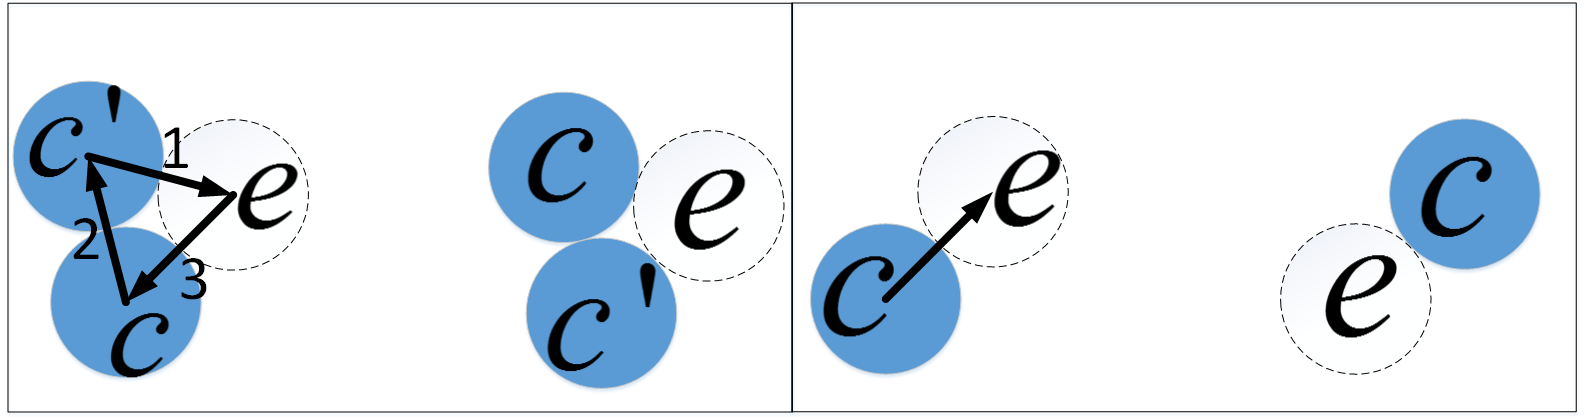
\includegraphics[width=0.5\linewidth]{figs/exchange.png}
\caption{\em This figure shows how Theorem \ref{thm:min} formulation can be used for moving/exchanging an element $\mathbf{c}$ with $\mathbf{c'}$.
The left picture shows how two non-empty elements can exchange their positions, based on the arrows. 
%The arrows and their associated numbers show the steps of exchange processing.
To move a non-empty element $\mathbf{c}$ to the other non-empty element $\mathbf{c'}$, it has to be an empty element to place the $\mathbf{c'}$ and then move $\mathbf{c}$ to the position $\mathbf{p_c'}$. This is shown as the third step with the arrow, which moves $\mathbf{c'}$ to $\mathbf{p_c}$. 
%In this manner, only $\mathbf{c}$ and $\mathbf{c'}$ exchange their positions and the rest of elements stay at their original positions.
%The right picture shows the other situation in which one of the elements is empty. To exchange their positions we only need to move the $\mathbf{c}$.
}
\label{fig:exchange}
\vspace*{-0.2in}
\end{figure}
Theorem \ref{thm:min} illustrates the spatial requirements in terms of packing to move an element.   
Assuming both nearby elements $\mathbf{c}$ and $\mathbf{c'}$ are not empty in terms of agents, if $\mathbf{c}$ wants to move to $\mathbf{p_c'}$ then there has to be at least one extra empty element $\mathbf{e}$ that connects both  $\mathbf{c}$ and  $\mathbf{c'}$ to complete the movement. The process involves moving $\mathbf{c'}$ to $\mathbf{p_e}$ in order to make its position free, and then moving $\mathbf{c}$ to $\mathbf{p_c'}$. The other situation arises when either $\mathbf{c}$ or $\mathbf{c'}$ represents empty position, in which case we can directly move the agent to an empty position. We illustrate both of these situations in Figure \ref{fig:exchange}.

Note that the above discussion assumes that $\mathbf{c}$ and $\mathbf{c'}$ are close to each other.
However, if $\mathbf{c}$ and $\mathbf{c'}$ are not in close proximity, then $\mathbf{c}$ has to repeatedly try such a movement to move towards $\mathbf{p_c'}$. During this computation (Algorithm 2, Steps 7 and 8), several agents are moved from their positions correspondingly. This could generate a problem because some of these agents being moved may already be at their goal positions. Ideally, we do not want to move such agents. 
%already, and thus they do not want to be interrupted by other agents' movements. 
Therefore, the design of an efficient algorithm is meant to move $\mathbf{c}$ to its goal position while keeping the irrelevant agents static. We present a general exchange algorithm. The input is two elements, and the output is these two elements exchanging their position while the rest of the agents are not moved. Fortunately, the exchange algorithms still meet the minimum spatial requirement in Theorem \ref{thm:min}. That is, the only single connected empty element is involved in the whole processing.

\vspace*{0.05in}
\begin{lemma}
Two elements that are in the same cluster can exchange their positions if and only if one of them is an empty element or there is the third empty element that connects at least one of them. 
\label{lem:min}
\end{lemma}
\vspace*{0.05in}

In the following part of this section we first introduce the intra-loop exchange algorithm and then deduct the inter-loop exchange algorithm.
\subsection{Intra-loop Exchange}
The goal of intra-loop exchange is to exchange two elements' positions that are in same loop $\mathbf{c} \in \mathbf{T}, \mathbf{c'} \in \mathbf{T} $. This needs an extra empty element in a nearby loop $\mathbf{e} \in \mathbf{T'}, \mathbf{T} \neq \mathbf{T'}$. The overall algorithm is shown in Algorithm \ref{algo:intraloop}. In line 1, $\mathbf{c}$ moves to the nearby empty position, thus emptying its own position. Note here that the loop $\mathbf{T}$ has an extra empty element because $\mathbf{c}$ has moved to anther loop. The algorithm moves all of the agents between $\mathbf{c}$ and $\mathbf{c'}$ by one step to adjust this empty element from $\mathbf{p_c}$ to $\mathbf{p_c'}$.
%and this processing is shown in line 2.
%In line 3-4, all of the agents $\in \mathbf{T}$ move around until $\mathbf{c}$ connects to $\mathbf{e}$. Then $\mathbf{e}$ moves to its original position. In line 3, $\mathbf{c'}$ moves to $\mathbf{p_e}$, and thus $\mathbf{T}$ has another empty element. Finally, we adjust the elements' position in the $\mathbf{T}$, make $\mathbf{c}$ takes $\mathbf{p_c'}$ and move $\mathbf{c'}$ to $\mathbf{p_c}$, which is taken by $\mathbf{e}$.
%After implementing the algorithm, only $\mathbf{c}$ and $\mathbf{c'}$ exchange their positions and, all of the rest of the agents stay at their primitive positions.
Figure \ref{fig:intra} shows such an example. 


\begin{figure}[!ht]
\centering
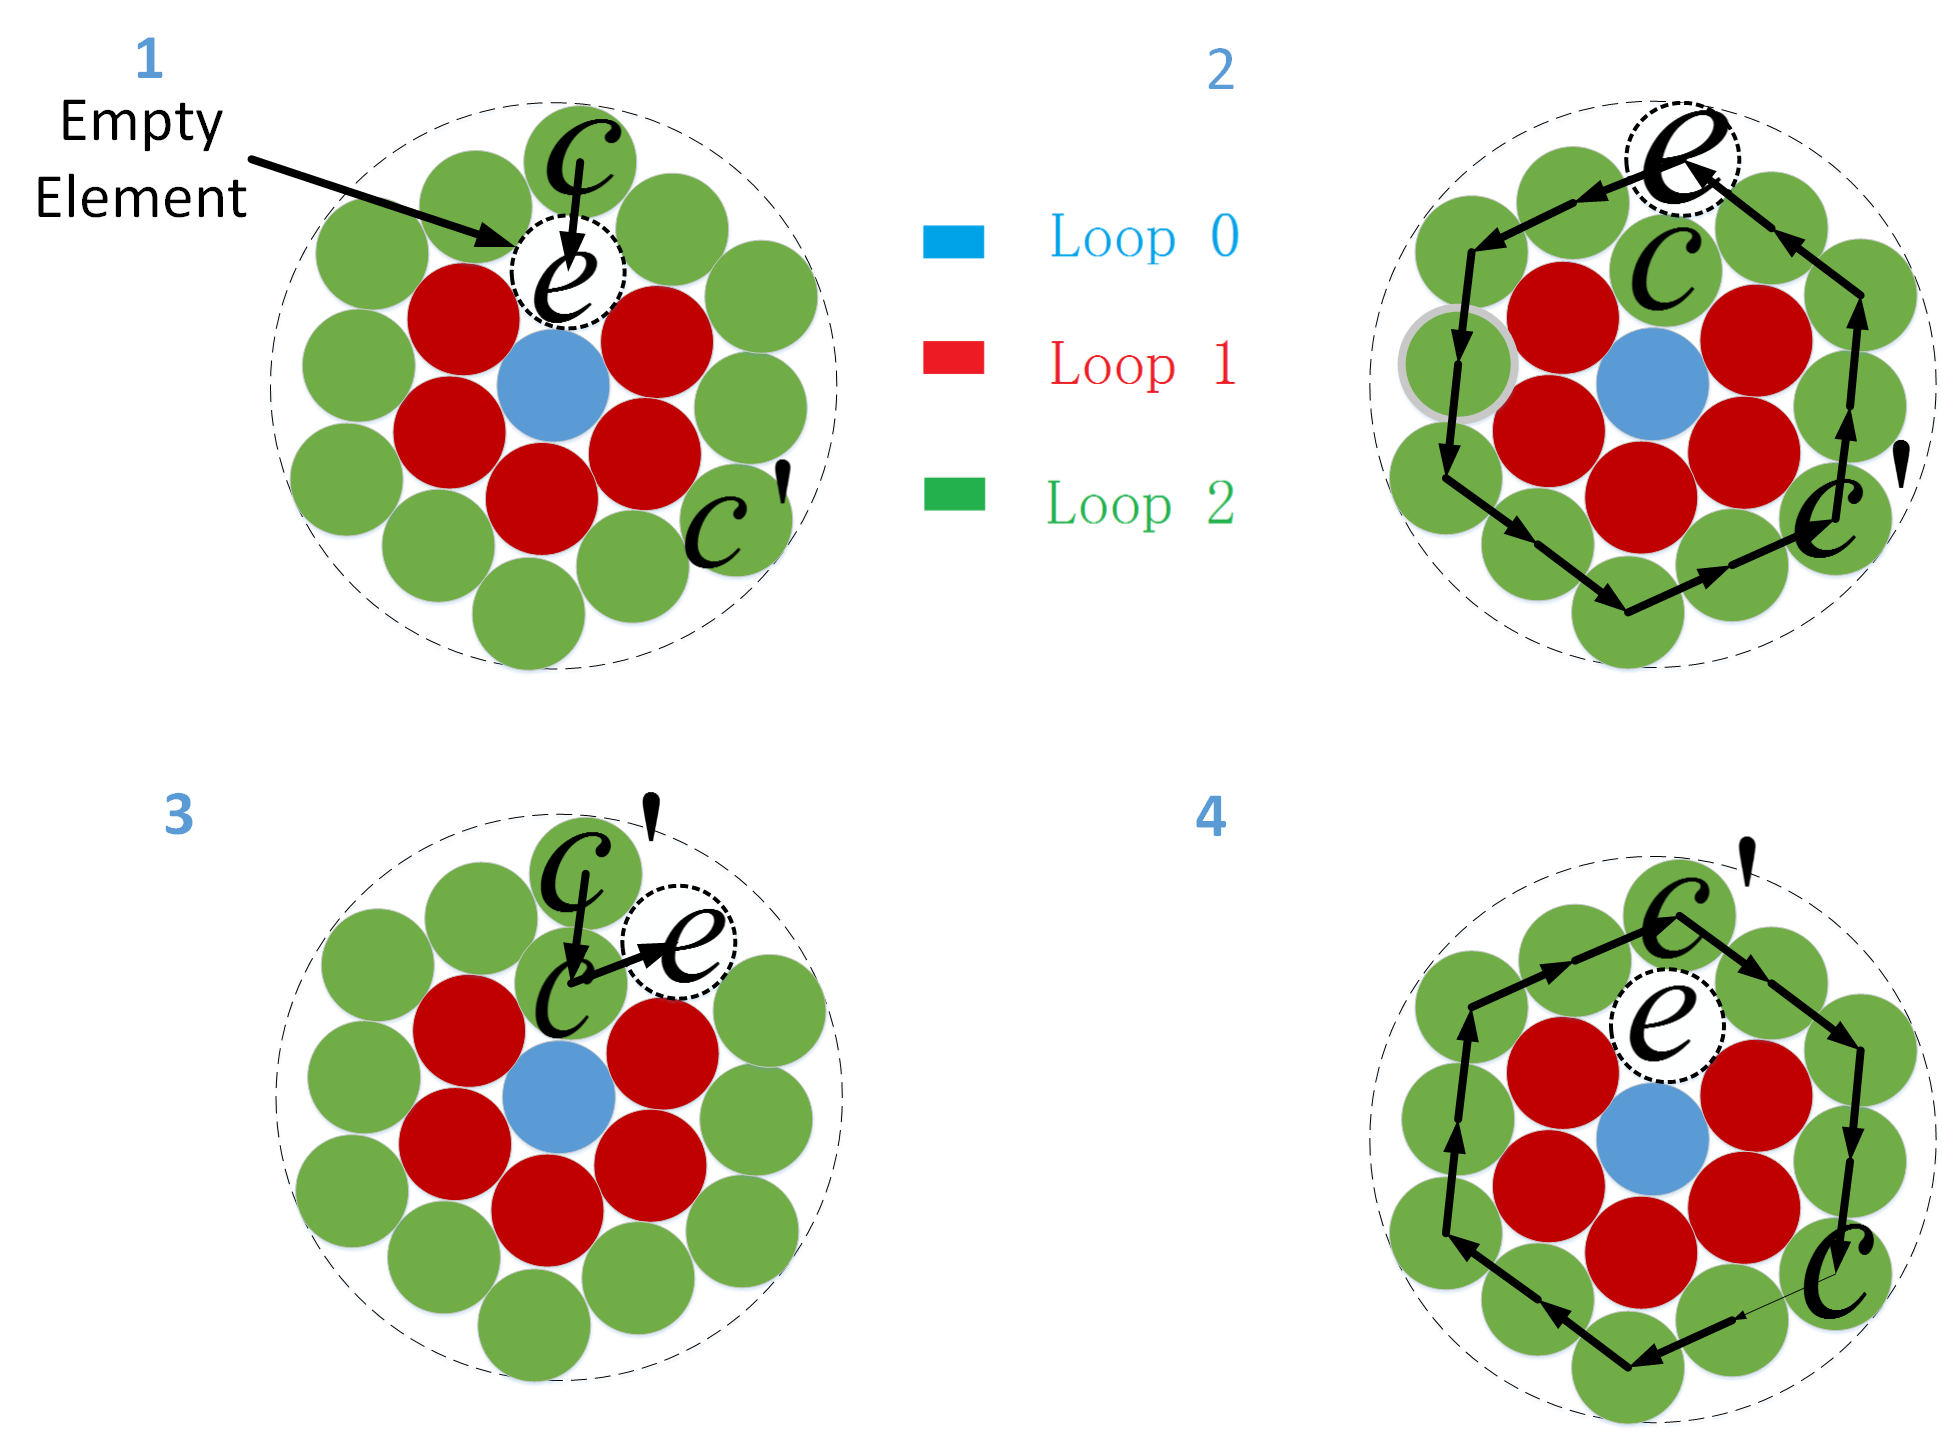
\includegraphics[width=0.7\linewidth]{figs/IntraMovement}
\caption{\em Sequences of intra-loop exchange processing: The upper left picture shows two elements $\mathbf{c} \in \mathbf{T}$ and $\mathbf{c'} \in \mathbf{T}$ with an empty element $\mathbf{e} \in \mathbf{T'}$. $\mathbf{c}$ moves to $\mathbf{p_e}$ (shown with an arrow) in this picture. In the upper right picture, all of the agents in $\mathbf{T}$ push each other to move simultaneously so that $\mathbf{c}$ could connect to $\mathbf{e}$ in $\mathbf{T}$. In the bottom left picture, $\mathbf{c}$ moves back to loop $\mathbf{T}$ and  $\mathbf{c'}$ temporarily move to loop $\mathbf{T'}$. In the bottom right picture, all the agents push each other back to their primitive position and  $\mathbf{c'}$ moves towards $\mathbf{T}$, thus finishing the exchange processing step.
%After the step in the bottom right picture,  $\mathbf{c}$ and $\mathbf{c'}$ exchange their positions and the rest of the elements stay at their current locations.
}
\label{fig:intra}
\vspace*{-0.2in}
\end{figure}


\begin{algorithm}[!th]
  \SetKwInOut{Input}{input}\SetKwInOut{Output}{output}
  \Input{An element $\mathbf{c} \in \mathbf{T}$ with its initial position $\mathbf{p_c}$ and the goal element $\mathbf{c'}$ position $\mathbf{p'}$ in the loop. An empty element, $\mathbf{e} \notin \mathbf{T}$, $\mathbf{e} \sim \mathbf{c}$
  }
  \Output{$\mathbf{c}$ and $\mathbf{c'}$ exchange their positions}
  \BlankLine
  Move $\mathbf{c}$ to $\mathbf{p_e}$;   Move $\mathbf{e}$ at $\mathbf{p_c}$ to $\mathbf{p_c'}$
  
  \While{ $\mathbf{c}$ and $\mathbf{c'}$ are not connected}{
  Simultaneously move all of elements $\in \mathbf{T}$.  
  }
  Move $\mathbf{c}$ to $\mathbf{c'}$'s nearby empty element\\
  
  Move $\mathbf{c'}$ to $\mathbf{p_e}$;  Move $\mathbf{c}$ to $\mathbf{p_c'}$ \\
  
  Move $\mathbf{c'}$ to $\mathbf{p_c}$ meanwhile return all agents $\in \mathbf{T}$ to their primitive positions\\
  
  \caption{Intra-loop Exchange: This is used in Algorithm 2, Steps 7 and 8.}
  \label{algo:intraloop}
\end{algorithm}


\subsection{Inter-cluster Exchange}
\begin{figure}[!ht]
\centering
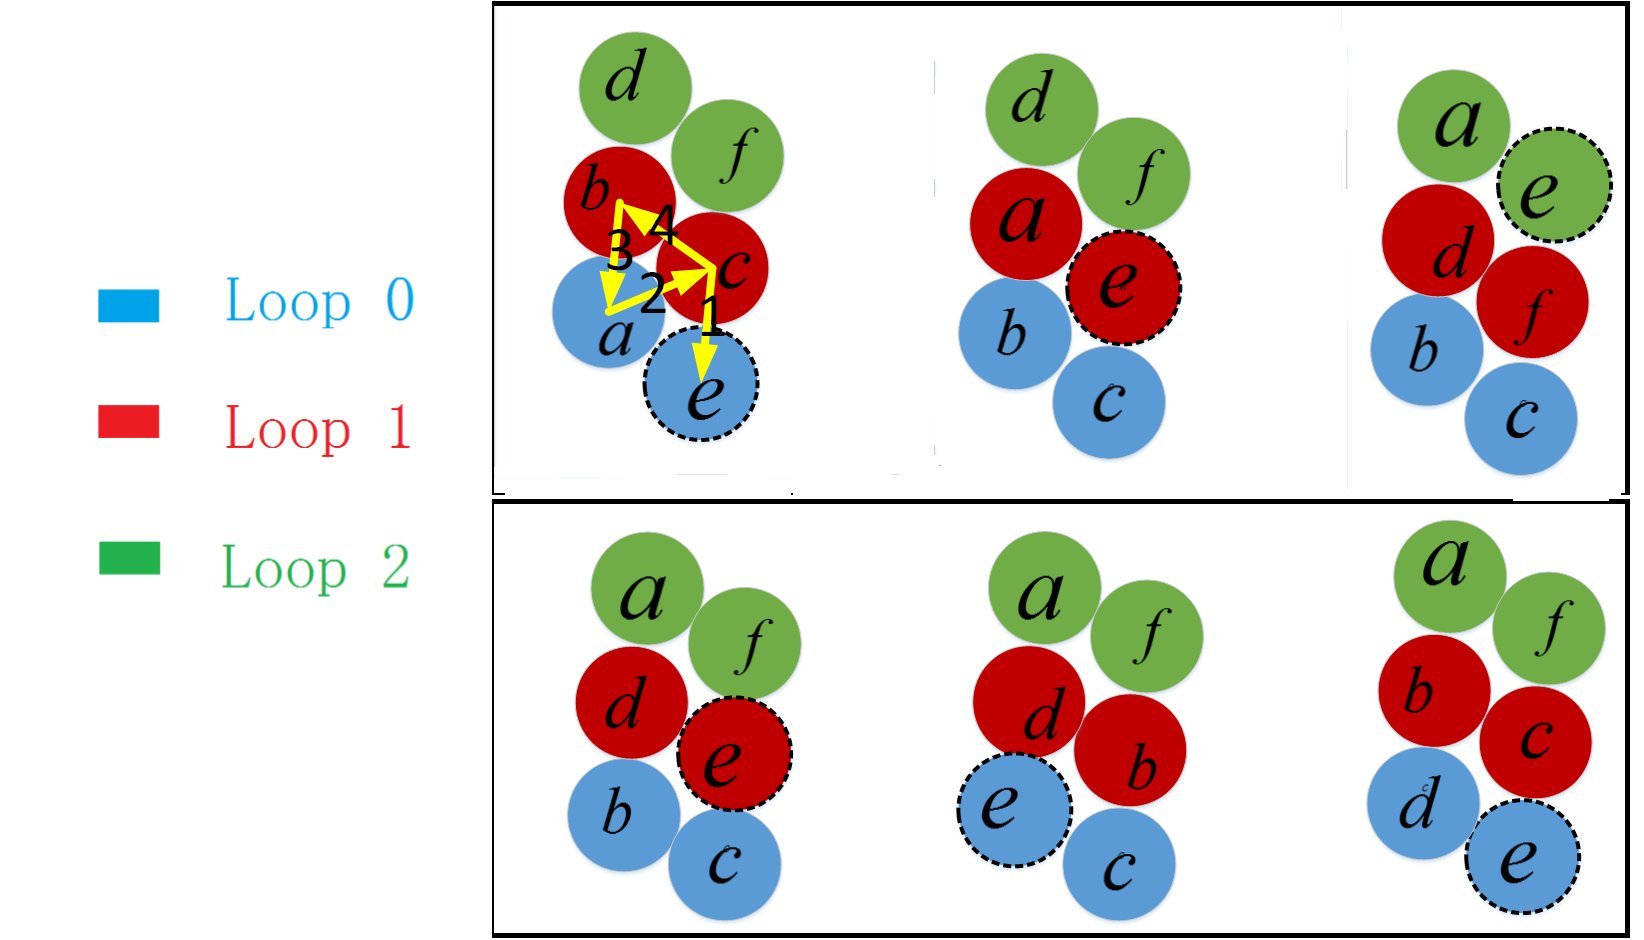
\includegraphics[width=0.6\linewidth]{figs/InterMovement}
\caption{\em This figure shows the sequence of how elements $\mathbf{a}$ and  $\mathbf{d}$ exchange their positions when they are not in the nearby loop. In this example, there are three loops, and we highlight each of them in different colors.
The upper row shows how $\mathbf{a}$ moves towards $\mathbf{p_d}$ with an empty element  $\mathbf{e}$. In each inter-loop movement, the pairs of elements are moved to another loop. After $\mathbf{a}$ reaches its goal, the two pairs of elements are moved away from their original loops. In the bottom row, the algorithm uses the same strategy as the left column to return $\mathbf{e}$ back to its original position. Throughout this process, every element that has been moved returns to its original position.}
\label{fig:inter}
\end{figure}


The inter-loop exchange represents two elements that are in different loops exchanging their positions. Again, we need an extra empty element $\mathbf{e}$ to connect one of the two elements $\mathbf{c}$ and $\mathbf{c'}$. 
We assume that they have the following relationships at the start state:
$ \{\mathbf{e}, \mathbf{c},\mathbf{c'} | \mathbf{e} \sim \mathbf{c}, \mathbf{e} \in \mathbf{T}, \mathbf{c} \in \mathbf{T}, \mathbf{c'} \in \mathbf{T'}, \mathbf{T'} \neq \mathbf{T} \}$. 
Our approach performs inter-loop exchanging, and we illustrate the approach in Figure \ref{fig:inter}.

%is shown in Algorithm \ref{algo:interloop}. 
%In lines 2-3, $\mathbf{c}$ moves to the nearby empty position $\mathbf{e}$ thus empty its position if in which has not one. 
%In lines 4-5, $\mathbf{c}$ keeps moving with $\mathbf{e}$ to $\mathbf{T'}$. This sub-algorithm is show in Algorithm \ref{algo:nearbyexchange}.
%Note that, in this processing, $\mathbf{c}$ moves with $\mathbf{e}$ in pairs.
%In line 6, $\mathbf{c}$ moves to $\mathbf{p_c'}$.  
%Lines 7-8 represent moving the $\mathbf{c'}$ with $\mathbf{e}$ to $\mathbf{p_c}$. This is the inverse processing of lines 4-5, and in this processing the elements moved during the processing of line 4-5 are returned to their primitive positions. 
%Finally, if $\mathbf{e}$ is borrowed from another place in the beginning, we use the intra-loop and inter-loop exchange algorithms to return it.
%In the intra-loop exchange algorithm, only $\mathbf{c}$ and $\mathbf{c'}$ exchange their positions.
%Figure \ref{fig:inter} shows an example to illustrate this computation. 


%\begin{algorithm}[!th]
%  \SetKwInOut{Input}{input}\SetKwInOut{Output}{output}
%  \Input{ $\mathbf{c} \in \mathbf{T}$, $\mathbf{c'}\in \mathbf{T'},  \mathbf{c''} \in \mathbf{T'}$, an empty element $\mathbf{e} \in \mathbf{T}$,
%  $\mathbf{T} \neq \mathbf{T'}$, $\mathbf{c} \sim \mathbf{c'} \sim \mathbf{e}$, $\mathbf{c'} \sim \mathbf{c'} \sim \mathbf{e}$}
%  \Output{$\mathbf{e}$ and $\mathbf{c}$ exchange their position with $\mathbf{c'}$ and $\mathbf{c''}$}
%  \BlankLine
  
%  \tcc{ $\mathbf{p_e}$, $\mathbf{p_c}$, $\mathbf{p_c'}$, $\mathbf{p_c''}$ are elements primitive positions, assume they are constant in following exchanges.}
%    $\mathbf{c'}$ moves to $\mathbf{p_e}$\\
%    $\mathbf{c}$ moves to $\mathbf{p_c'}$\\
%    $\mathbf{c'}$ moves to $\mathbf{p_c}$\\
%    $\mathbf{c''}$ moves to $\mathbf{p_e}$\\
 
%  \caption{Neighboring Loops Exchange: This is used in Algorithm 4, Step 5, 7 and 10.}
%  \label{algo:nearbyexchange}
%
%\end{algorithm}
\begin{figure}[!ht]
\centering
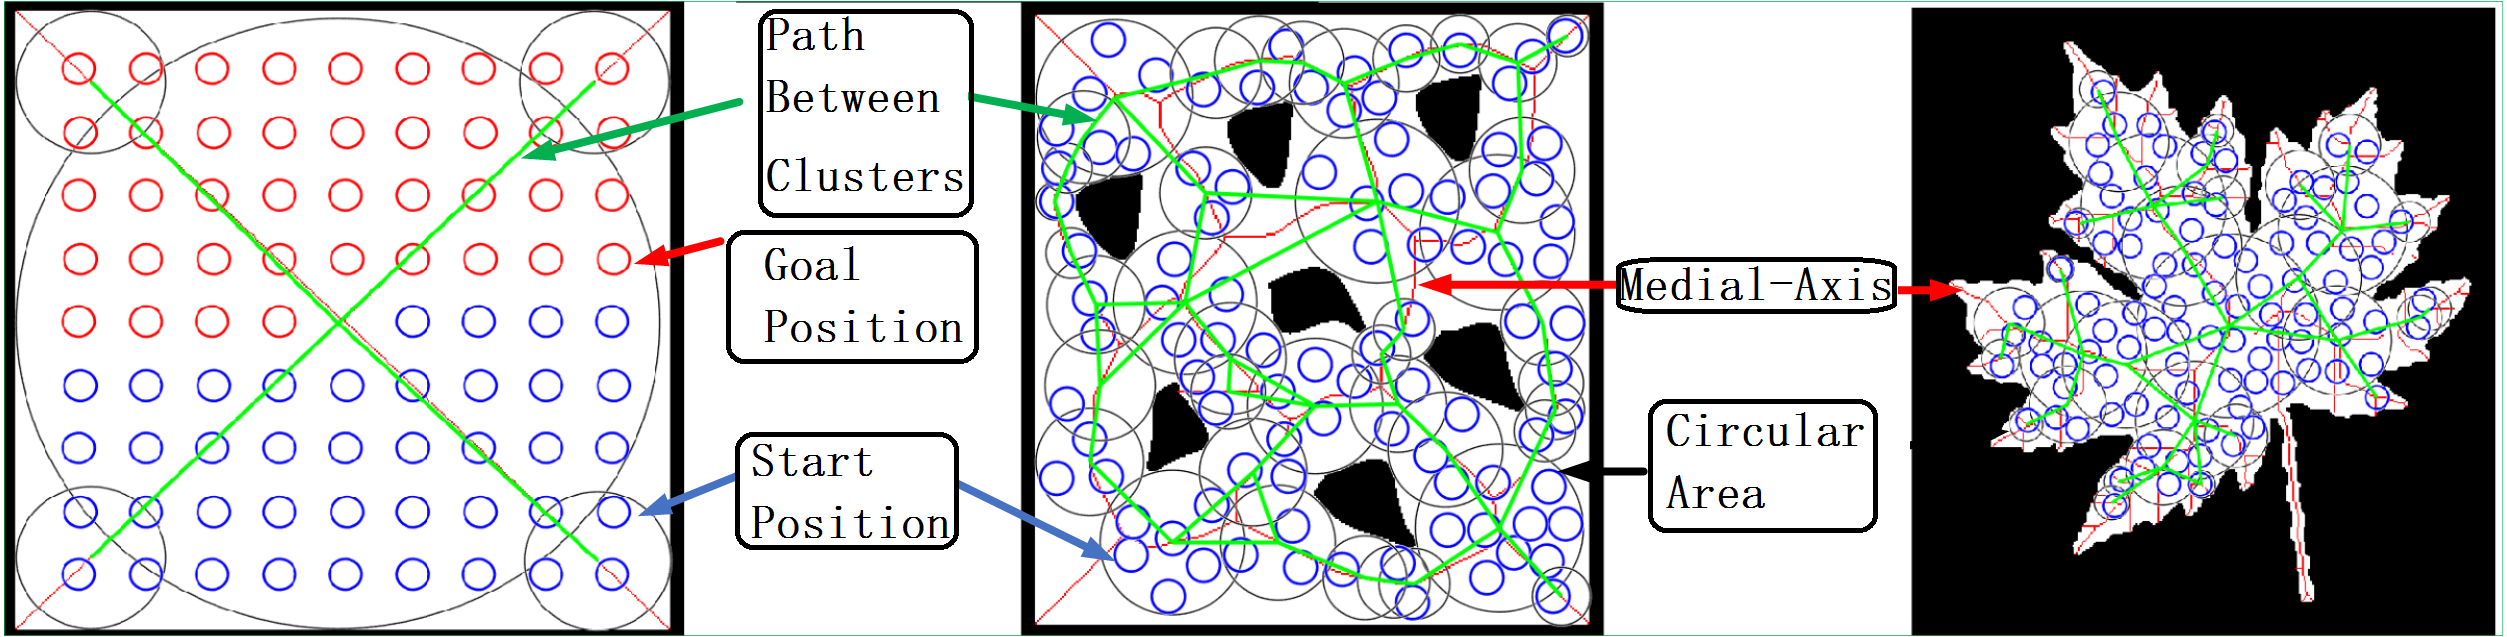
\includegraphics[width=\linewidth]{figs/Benchmarks/benchmark.png}
\caption{\em We show three challenging benchmarks with $40-100$ agents, where techniques based on decentralized methods may not work well. We highlight the start positions (blue agents), the goal positions (red agents) and the medial-axis, the path between the clusters (green). Our algorithm can compute the paths for all agents in $3-8$ seconds.}
\vspace*{-0.3in}
\label{fig:benchmarks}
\end{figure}





%\section{Resolution-Completeness}

In this section, we present an algorithm for an agent's intra-cluster movements and prove its completeness. Next we present a criterion to connect all possible clusters.
%To extend this result into the global environment, we present another algorithm with a criterion to connect all of the possible clusters together. 
Based on checking whether a cluster $\mathbf{C}$ can be connected with another cluster whose incident circle $A(\mathbf v,ran)$ includes the goal position of an agent $\mathbf{a} \in \mathbf{C}$, we conclude whether there is path for $\mathbf{a}$ to reach its goal. 
 
 %\begin{algorithm}[!th]
  % \SetKwInOut{Input}{input}\SetKwInOut{Output}{output}
  % \Input{A set of agents in an cluster $\mathbf{a_0, a_1, ..., a_n \in A}$, assume both of their start positions
 %  and goal positions are in its incident circle  $p_0, p_1, ..., p_n \in  A(v,ran), p'_0, p'_1, ..., p'_n \in A(v,ran)$ }
 %  \Output{agents are moved to their individual goals. }
 %  \BlankLine
 % \tcc{ }
 %  \For{$\mathbf{a_i}, i = 0:n$}{
 %    \If{$\mathbf{a_i}$ does not connect with an empty element $\mathbf e \in A$}{
  %       Exchange an $\mathbf e \in A$ to the nearby position of $\mathbf{a_i}$ \\
 %    }
  %   \If{$\mathbf{p_i} \in \mathbf{T}$ and $\mathbf{p'_i} \in \mathbf{T}$}{
  %       Do intra-loop exchange to move $\mathbf{a_i}$ to $\mathbf{p'_i}$\\
  %   }
  %   \Else{
  %       Do inter-loop exchange to move $\mathbf{a_i}$ to $\mathbf{p'_i}$\\
 %    }
 %  }
  % \caption{Intra-movement algorithm}
  % \label{algo:intramovement}
 %\end{algorithm}
 
\subsection{Completeness of Intra-cluster Computation}


We extend Lemma \ref{lem:min} to the following lemma, which gives the minimum spatial requirement to implement an exchange algorithm inside of a circle.

\vspace*{.05in}
\begin{lemma}
Assume a cluster $\mathbf{A}$ and its incident circle $A(\mathbf v,ran)$ is non-full. $\forall \mathbf{a} \in \mathbf{A}$, we can find a complete path from its start position $\mathbf{p_a} \in A(\mathbf v,ran)$ to the goal position $\mathbf{p_a'} \in A(\mathbf v,ran)$ and we refer to that cluster $\mathbf{A}$ is complete. 
\label{lem:intra-unit complete}
\end{lemma}


\subsection{Connect Clusters}
So far we have shown that for any agent, if both its start position and goal position are in a non-full circle, then our algorithm can find a path to reach its goal. 
In this section, we present an algorithm that connects such clusters together to extend the inter-loop exchange algorithm to  inter-cluster level.
We show that all the agents can move around in the connected cluster. Based on this criterion, the problem of path existence and computation for an agent reduces to checking whether the agent's goal position is within the connected cluster.
%and their relevant area.
%With this criterion, it turns out that checking if there exists a solution to move an agent to its goal has been changed into checking whether the agent's goal position is at a connected cluster. 


\begin{theorem}
Suppose we have a path $\mathcal{P}\mathbf{(v, v')} \subseteq \mathcal{G}$, that connects two areas $A(\mathbf v,ran)$ and $A(\mathbf v',ran')$ with their corresponding clusters $\mathbf{A}$ and $\mathbf{A'}$.
Then, if $\{\mathcal{P}\mathbf{(v, v')}\ |\ \forall A(\mathbf p,ran''),\ \mathbf{p} \in \mathcal{P}\mathbf{(v, v')},\ \forall \mathbf{a} \notin \mathbf{A} \cup \mathbf{A'},\ \mathbf{a} \cap A(\mathbf p,ran) = \varnothing\}$, we label the path $\mathcal{P}\mathbf{(v, v')}$ as clean.
\label{them:clean}
\end{theorem}

Note that we mentioned that $\mathcal{G}$ does not include the points whose incident circles' radius are smaller than the agent's radius. Thus, for any incident circle of $\mathcal{P}\mathbf{(v, v')}$, it has the capability to accommodate at least one agent. 
With this assumption, Theorem \ref{them:clean} can be explained as, if $A(\mathbf v', ran)$ is non-full, then it has an element $ \exists \mathbf{c} \in A(\mathbf v,ran)$ that can move along $\mathcal{P}\mathbf{(v, v')}$ to reach $A(\mathbf v', ran)$ and it does not touch any other cluster's agent during this movement. 

\begin{definition}
For two areas $A(\mathbf v, ran)$ and $ A(\mathbf v', ran')$, we call them connected if there exists a clean path $\mathcal{P(\mathbf v,\mathbf v')}$ that connects them. 
\label{def:connect}
\end{definition}


\begin{lemma}
If two areas $A(\mathbf v, ran)$ and $A(\mathbf v', ran')$ are connected, and at least one of them is non-full, then all of their elements can reach any position if $ \mathbf{p} \in A(\mathbf v, ran) \cup A(\mathbf v', ran')$ .
\label{lem:intertcluster}
\end{lemma}


\begin{lemma}
Suppose all clusters are connected. If there is one cluster whose area is not-full, or we can remove an agent from a full area to a new location without impacting the clearance of all the paths between the clusters, then we can find a solution to move all agents to their goals. Otherwise, there is no solution (i.e. path) for the current scenario.
\label{lem:complete}
\end{lemma}
The last lemma proves the completeness of our algorithm.
%\section{Analysis}
\vspace*{+0.15in}
In this section, we analyze the computational complexity of our algorithm. 
The overall algorithm includes two parts, medial-axis computation and multi-agent motion planning. Since we use a sample-based approach to compute the medial axis, its complexity is  $O(klogk)$  ~\cite{giesen2012medial}, for $k$ samples.
%Because we use the sampling methods to compute the medial-axis in this paper, the computational complexity is relevant to the number of samples. Assume the number of samples is $k$; then the complexity is $O(klogk)$  ~\cite{giesen2012medial}.
For path computation, assume we have $n$ agents and we move one agent at a time and the agent's movement takes $m$ steps to reach the goal position. In the worst case, $n-1$ agents may have to move temporarily for this one agent and that takes $a$ steps. As a result, the overall complexity is bounded by $O(a n^2)$. So the overall complexity is bounded by $O(klogk + an^2)$.
\vspace*{+0.15in}
%then the agent's movement costs $m$ steps to reach its goal position. However, the rest of the agents would be temporarily moved, as in the algorithms that we illustrated. Assume for each agent's movements(reach its goal position, there are at most $n-1$ agents would be interrupted and for return to their primitive positions, it will cost $a$ steps, then the computational complexity is $O(an^2)$. If we add two steps together, the overhead is $O(klogk + an^2)$, where $N$ is the number of samples on the obstacle's boundary.

%\section{Implementation and Performance}
\begin{table}[t]
\centering{}%
\begin{tabular}{|c|c|c|c|c|c|}
\hline

\multicolumn{1}{|c|}{} & \# Agents & MAT  & Clusters  & Movements & Total  \\ \hline
 \#1 &40& 0.24 & 0.410  &2.35 &  3.001 \tabularnewline
 \#2 &100& 0.315  &0.398& 7.43 & 8.143\tabularnewline
 \#3 &100& 0.270 &0.331& 7.21 &  7.811\tabularnewline
\hline
\end{tabular}
\caption{\em The performance of our algorithm on three challenging benchmarks (Benchmark \#1, \#2, \#3. We highlight the running time (in seconds) of medial axis computation (MAT), cluster computation (Clusters), agent movements (Movement) and the total running time.}
\vspace{-0.5cm}
\label{tab:benchmark}
\end{table}
In this section, we describe our implementation and highlight the
performance on three different benchmarks. In the first benchmark, we compare
our approach with a recent algorithm on continuous space centralized planning.
~\cite{DBLP:journals/corr/SoloveyYZH15}. The other two benchmarks represent challenging scenarios.
%in the table \ref{tab:benchmark}, we call it \emph{Optimal Guarantee}. We then implement other two benchmarks with a large number(100) of agents to show the robust of our algorithm. 
We have implemented our algorithms in C++
on a Intel Core i7 CPU running at 3.30GHz with 16GB of RAM
and running Windows 7. All of the timing results are generated on
a single core.
%In all of our benchmarks,
%we use red lines and black circles to mark the medial-axis and a clustering result. We highlight the graph paths of clusters as green lines. 
All of the running times are shown in the table \ref{tab:benchmark} and we show the time spent in different stages of the algorithm.
%separate the result to a calculation of agents' movements and pre-computation stages. The calculation of agents' movements includes the overhead of calculating all agents' movements to move them to their individual goals. The pre-computation stage includes all medial-axis calculation, clustering agents, tight pattern checking, and the overhead of building the connections of clusters. 

\noindent {\bf Benchmark 1:} We simulate the scenario shown in~\cite{DBLP:journals/corr/SoloveyYZH15}.
There are $40$ agents in a rectangle scenario and we highlight their start and goal positions. We can compute all the paths in $3$ seconds, as opposed to taking  $311$  seconds in ~\cite{DBLP:journals/corr/SoloveyYZH15}.
%start positions and goal positions with red and blue color respectively. The first picture of Figure ~\ref{fig:benchmarks} shows the scenario. Our method does not target on finding the optimal paths for all agents, and our running time outperforms their results.  

\noindent {\bf Benchmark 2:} We simulate a rectangle-shaped scenario with some complex-shaped obstacles. 
There are $100$ agents in this scenario. Each agent randomly selects another agents' start position as its goal position. We assume that the agents' goal positions are not overlapping. We can compute collision free paths in about $8$ sec.
%The Second picture of Figure ~\ref{fig:benchmarks} shows the scenario. 

\noindent {\bf Benchmark 3:}
We simulate a leaf-like scenario which has a complex boundary shape with a lot of edges. Prior methods will not work in such a scenario. %complicated edges. 
There are $100$ agents in this scene and each agent randomly pick another agents' start position as its goal position. We assume that the goal positions are not overlapping and our algorithm takes about $8$ seconds.
%agents' goals are not overlapping. The right-most picture of Figure ~\ref{fig:benchmarks} shows the scenario. 


\section{ Limitations and Future Work}

We present a novel method to compute collision-free paths for the homogeneous multi-agent motion planning with arbitrarily-shaped obstacles. We use the medial-axis of the workspace and our approach is resolution-complete. To the best of our knowledge, this is the first approach that can provide such guarantees for arbitrarily-shaped obstacles and we observe up to $100$X speedup over prior methods.
%Compared to former centralized methods, we are the first method that can handle the arbitrarily-shaped obstacles while giving completeness.
%Our method can be classified to geometric decomposition algorithms. Unlike previous methods, our method is fast and the computational complexity is not limited to the polygonal shape of %obstacles.
Our approach has some limitations. It is limited to homogeneous disc-like agents and does not take into account dynamics constraints. Furthermore, we can't provide any optimality guarantees.
%Currently, our method can only handle the agents without considering their dynamic constraints, and the shape of the agent is limited to circle. Additionally, we only give one existed solution without consider the optimal one. 
There are many avenues for future work. In addition to overcoming
these limitations, we would like to design new methods based on medial-axis to simulate human-like behaviors or planning for high-DOF agents. Instead of moving one agent at a time, we would like to develop approaches that allow multiple agents to move simultaneously in complex scenarios.
%in dense crowd scenarios.
%Finally, instead of the algorithm that moves one agent at a time, we would like to moving multiple agents in once and simulating hundreds of agents in complex scenarios.  


\appendices
\section{Proof of the First Zonklar Equation}
Appendix one text goes here.

% you can choose not to have a title for an appendix
% if you want by leaving the argument blank
\section{}
Appendix two text goes here.


% use section* for acknowledgment
\section{Acknowledgment}
The authors would like to thank...


% Can use something like this to put references on a page
% by themselves when using endfloat and the captionsoff option.
\ifCLASSOPTIONcaptionsoff
  \newpage
\fi



\bibliographystyle{IEEEtran}
\bibliography{reference}



%\begin{thebibliography}{1}
%
%\bibitem{IEEEhowto:kopka}
%H.~Kopka and P.~W. Daly, \emph{A Guide to \LaTeX}, 3rd~ed.\hskip 1em plus
%  0.5em minus 0.4em\relax Harlow, England: Addison-Wesley, 1999.
%
%\end{thebibliography}



\end{document}


